\documentclass[11pt]{article}

\usepackage{times}
\usepackage{epsf}
\usepackage{epsfig}
\usepackage{amsmath, alltt, amssymb, xspace}
\usepackage{wrapfig}
\usepackage{fancyhdr}
\usepackage{url}
\usepackage{verbatim}
\usepackage{fancyvrb}

\usepackage{subfigure}
\usepackage{cite}
%\usepackage{cases}
%\usepackage{ltexpprt}
%\usepackage{verbatim}

%\topmargin      -0.70in  % distance to headers
%\headheight     0.2in   % height of header box
%\headsep        0.4in   % distance to top line
%\footskip       0.3in   % distance from bottom line

% Horizontal alignment
\topmargin      -0.50in  % distance to headers
\oddsidemargin  0.0in
\evensidemargin 0.0in
\textwidth      6.5in
\textheight     8.9in 


%\centerfigcaptionstrue

%\def\baselinestretch{0.95}


\newcommand\discuss[1]{\{\textbf{Discuss:} \textit{#1}\}}
%\newcommand\todo[1]{\vspace{0.1in}\{\textbf{Todo:} \textit{#1}\}\vspace{0.1in}}
\newtheorem{problem}{Problem}[section]
%\newtheorem{theorem}{Theorem}
%\newtheorem{fact}{Fact}
\newtheorem{define}{Definition}[section]
%\newtheorem{analysis}{Analysis}
\newcommand\vspacenoindent{\vspace{0.1in} \noindent}

%\newenvironment{proof}{\noindent {\bf Proof}.}{\hspace*{\fill}~\mbox{\rule[0pt]{1.3ex}{1.3ex}}}
%\newcommand\todo[1]{\vspace{0.1in}\{\textbf{Todo:} \textit{#1}\}\vspace{0.1in}}

%\newcommand\reducespace{\vspace{-0.1in}}
% reduce the space between lines
%\def\baselinestretch{0.95}

\newcommand{\fixmefn}[1]{ \footnote{\sf\ \ \fbox{FIXME} #1} }
\newcommand{\todo}[1]{
\vspace{0.1in}
\fbox{\parbox{6in}{TODO: #1}}
\vspace{0.1in}
}

\newcommand{\mybox}[1]{
\vspace{0.2in}
\noindent
\fbox{\parbox{6.5in}{#1}}
\vspace{0.1in}
}


\newcounter{question}
\setcounter{question}{1}

\newcommand{\myquestion} {{\vspace{0.1in} \noindent \bf Question \arabic{question}:} \addtocounter{question}{1} \,}

\newcommand{\myproblem} {{\noindent \bf Problem \arabic{question}:} \addtocounter{question}{1} \,}


\newcommand{\copyrightnoticeA}[1]{
\vspace{0.1in}
\fbox{\parbox{6in}{\small Copyright \copyright\ 2006 - 2014\ \ Wenliang Du, Syracuse University.\\ 
      The development of this document is partially funded by 
      the National Science Foundation's Course, Curriculum, and Laboratory 
      Improvement (CCLI) program under Award No. 0618680 and 0231122. 
      Permission is granted to copy, distribute and/or modify this document
      under the terms of the GNU Free Documentation License, Version 1.2
      or any later version published by the Free Software Foundation.
      A copy of the license can be found at http://www.gnu.org/licenses/fdl.html.}}
\vspace{0.1in}
}


\newcommand{\copyrightnotice}[1]{
\vspace{0.1in}
\fbox{\parbox{6in}{\small Copyright \copyright\ 2006 - 2014\ \ Wenliang Du, Syracuse University.\\
      The development of this document is/was funded by three grants from
      the US National Science Foundation: Awards No. 0231122 and 0618680 from
      TUES/CCLI and  Award No. 1017771 from Trustworthy Computing.
      This lab was imported into the Labtainer framework by the Naval Postgraduate 
      School, Center for Cybersecurity and Cyber Operations under National Science 
      Foundation Award No. 1438893.
      Permission is granted to copy, distribute and/or modify this document
      under the terms of the GNU Free Documentation License, Version 1.2
      or any later version published by the Free Software Foundation.
      A copy of the license can be found at http://www.gnu.org/licenses/fdl.html.}}
\vspace{0.1in}
}

\newcommand{\copyrightnoticeB}[1]{
\vspace{0.1in}
\fbox{\parbox{6in}{\small Copyright \copyright\ 2006 - 2014\ \ Wenliang Du, Syracuse University.\\
      The development of this document is/was funded by the following grants from
      the US National Science Foundation: No. 0231122, 0618680, and 1303306.
      Permission is granted to copy, distribute and/or modify this document
      under the terms of the GNU Free Documentation License, Version 1.2
      or any later version published by the Free Software Foundation.
      A copy of the license can be found at http://www.gnu.org/licenses/fdl.html.}}
\vspace{0.1in}
}


\newcommand{\nocopyrightnotice}[1]{
\vspace{0.1in}
\fbox{\parbox{6in}{\small  
      The development of this document is funded by 
      the National Science Foundation's Course, Curriculum, and Laboratory 
      Improvement (CCLI) program under Award No. 0618680 and 0231122. 
      Permission is granted to copy, distribute and/or modify this document.
      }}
\vspace{0.1in}
}

\newcommand{\idea}[1]{
\vspace{0.1in}
{\sf IDEA:\ \ \fbox{\parbox{5in}{#1}}}
\vspace{0.1in}
}

\newcommand{\questionblock}[1]{
\vspace{0.1in}
\fbox{\parbox{6in}{#1}}
\vspace{0.1in}
}


\newcommand{\minix}{{\tt Minix}\xspace}
\newcommand{\unix}{{\tt Unix}\xspace}
\newcommand{\linux}{{\tt Linux}\xspace}
\newcommand{\ubuntu}{{\tt Ubuntu}\xspace}
\newcommand{\selinux}{{\tt SELinux}\xspace}
\newcommand{\freebsd}{{\tt FreeBSD}\xspace}
\newcommand{\solaris}{{\tt Solaris}\xspace}
\newcommand{\windowsnt}{{\tt Windows NT}\xspace}
\newcommand{\setuid}{{\tt Set-UID}\xspace}
%\newcommand{\smx}{{\tt Smx}\xspace}
\newcommand{\smx}{{\tt Minix}\xspace}
\newcommand{\relay}{{\tt relay}\xspace}
\newcommand{\isys}{{\tt iSYS}\xspace}
\newcommand{\ilan}{{\tt iLAN}\xspace}
\newcommand{\iSYS}{{\tt iSYS}\xspace}
\newcommand{\iLAN}{{\tt iLAN}\xspace}
\newcommand{\iLANs}{{\tt iLAN}s\xspace}
\newcommand{\bochs}{{\tt Bochs}\xspace}

\newcommand\FF{{\mathcal{F}}}

\newcommand{\argmax}[1]{
\begin{minipage}[t]{1.25cm}\parskip-1ex\begin{center}
argmax
#1
\end{center}\end{minipage}
\;
}

\newcommand{\bm}{\boldmath}
\newcommand  {\bx}    {\mbox{\boldmath $x$}}
\newcommand  {\by}    {\mbox{\boldmath $y$}}
\newcommand  {\br}    {\mbox{\boldmath $r$}}


%\pagestyle{fancyplain}
%\lhead[\thepage]{\thesection}      % Note the different brackets!
%\rhead[\thesection]{SEED Laboratories}
%\lfoot[\fancyplain{}{}]{Syracuse University} 
%\cfoot[\fancyplain{}{}]{\thepage} 

\newcommand{\tstamp}{\today}   
%\lhead[\fancyplain{}{\thepage}]         {\fancyplain{}{\rightmark}}
%\chead[\fancyplain{}{}]                 {\fancyplain{}{}}
%\rhead[\fancyplain{}{\rightmark}]       {\fancyplain{}{\thepage}}
%\lfoot[\fancyplain{}{}]                 {\fancyplain{\tstamp}{\tstamp}}
%\cfoot[\fancyplain{\thepage}{}]         {\fancyplain{\thepage}{}}
%\rfoot[\fancyplain{\tstamp} {\tstamp}]  {\fancyplain{}{}}

\pagestyle{fancy}
%\lhead{\bfseries Computer Security Course Project}
\lhead{\bfseries SEED Labs}
\chead{}
\rhead{\small \thepage}
\lfoot{}
\cfoot{}
\rfoot{}

\usepackage{listings}
\usepackage{color}

\definecolor{dkgreen}{rgb}{0,0.6,0}
\definecolor{gray}{rgb}{0.5,0.5,0.5}
\definecolor{mauve}{rgb}{0.58,0,0.82}

\lstset{frame=tb,
  language=C,
  aboveskip=3mm,
  belowskip=3mm,
  showstringspaces=false,
  columns=flexible,
  basicstyle={\small\ttfamily},
  numbers=none,
  numberstyle=\tiny\color{gray},
  keywordstyle=\color{blue},
  commentstyle=\color{dkgreen},
  stringstyle=\color{mauve},
  breaklines=true,
  breakatwhitespace=true,
  tabsize=3
}



\begin{document}

\begin{center}
{\LARGE ICS Network Traffic}
\vspace{0.1in}\\
\end{center}


\section{Overview}
This exercise uses the GrassMarlin network traffic tool to
observe network activity that you generate while working
with a simple PLC device.  
GrassMarlin is a software tool released by the NSA that provides a method for discovering and cataloging
Supervisory Control \& Data Acquisition (SCADA) and Industrial Control System (ICS) hosts on IP-based
networks.  

This exercise assumes that student has performed the {\tt softplc2} lab.
Preliminary steps taken by the student are similar to those from that lab.

\section{Lab Environment}
This lab runs in the Labtainer framework,
available at http://nps.edu/web/c3o/labtainers.
That site includes links to a pre-built virtual machine
that has Labtainers installed, however Labtainers can
be run on any Linux host that supports Docker containers.

From your labtainer-student directory start the lab using:
\begin{verbatim}
    labtainer plc-traffic
\end{verbatim}
A link to this lab manual will be displayed, along with a link to the GrassMarlin 
user guide.

\section{Lab topology}
The lab includes four components as shown in Figure \ref{fig:topology}:
\begin{itemize}
\item \textbf{Slave Device} A simple slave device containing two buttons and a lamp.  The device has an
ethernet interface via which it is connected to a PLC using Modbus TCP/IP.
\item \textbf{PLC} A programmable logic controller implemented using the OpenPLC Soft-PLC implementation
on a Linux based computer.  The PLC is connected to the slave device via Modbus TCP/IP over ethernet.
The PLC has a separate ethernet connection to an HMI computer.
For convenience of the lab, the PLC computer includes Wireshark and will be used to capture, review and
replay network traffic between the PLC and the slave device.  

\item \textbf{HMI} A computer that interacts with the PLC using a web browser to load programs and monitor its operation.  This
computer also contains an OpenPLC Editor for constructing programs using ``Ladder Logic'' (LD).

\item \textbf{NETMON} A device that has taps on both of the networks, and collects PCAPs from those networks into files within its {\tt /taps} 
directory.
\end{itemize}

The PLC and the slave device communicate via Modbus TCP/IP, with the PLC acting as the master.  
The HMI component in this topology does not use Modbus, rather it simply interacts with the PLC via the
PLC's web server.
\begin{figure}[H]
\begin{center}
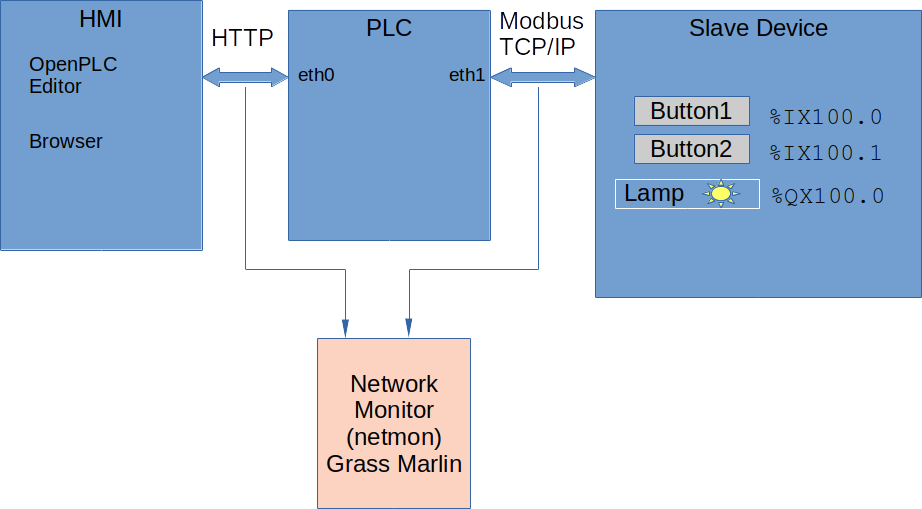
\includegraphics [width=0.8\linewidth]{plc-traffic.png}
\end{center}
\caption{Soft PLC Lab Topology}
\label{fig:topology}
\end{figure}

\section{Tasks}
In this lab, you will upload a simple ``hello world'' program
from the HMI to the PLC and use it to control the slave device.  You will use GrassMarlin to view the resulting traffic.

\subsection{Explore}
Find the {\tt Physical Board} window.  This is your virtual slave device.  Click the two buttons and confirm nothing happens.
This board is connected to the PLC via Modbus TCP/IP, however the PLC is not yet running and is not yet programmed.

\subsection{Upload and run PLC program}
In this task, you will deploy an existing ``hello world'' program onto the PLC and demonstrate its use.

\subsection{Start the PLC user interface \& Explore}
On the HMI terminal, use the firefox browser to access the PLC using port 8080:
\begin{verbatim}
    firefox plc:8080 &
\end{verbatim}
\noindent Login to the PLC through the browser with {\tt openplc} as the username and password.  
You should now see the Open PLC web page that controls the PLC.  Click the {\tt Slave Devices} button
on the left.  And double click on the {\tt myserver entry}.  This is the slave device that your PLC program will control.
Note we define only 3 bits to control the slave device.  Two bits as \textit{Descrete Inputs} for two buttons (only one 
of which is initially used), an one bit for the lamp as \textit{Coils}.
Make a note of the slave device IP address and  the port number used to communicate using Modbus.

\subsubsection{Upload the ST program to the PLC}
Select {\tt Programs} on the left pane and use the
{\tt Browse} button to locate the {\tt hello.st} file.  Then upload it to the PLC.  Provide a {\tt Name} in the resulting form
and press the {\tt Upload program} button.  Note the program is compiled on the PLC and results are displayed in
the browser.  Then click the {\tt Go to Dashboard} button.

The PLC now has your {\tt hello world} program loaded, but the PLC is not yet running.
Click the {\tt Start PLC} button.  Once the PLC is started, click the Monitoring button.

\subsubsection{Test the PLC program}
On the Physical Board, click button1.  The light bulb should come on for a few seconds.  Observe the indicators on the browser
Monitoring page.  

Stop the PLC and close the browser.

\subsection{View traffic}
You will now view the traffic that your activity has generated.  The {\tt netmon} component has taps into both of your networks, and collects 
traffic into pcap files stored in the {\tt /taps} directory.  

These steps are performed from the {\tt netmon} computer.
\begin{itemize}
\item Start the program with the command: {\tt grassmarlin}.  If the resulting GUI is not readable 
(i.e., is a black or blank window), close it and restart the program.
\item From the ``File'' menu, select ``Import Files'' and use the ``Add Files'' button and the file
browser to add the two PCAP files found in {\tt /taps}.  Then use the ``Import Selected'' button
on the ``Import'' dialog to import those files.  It may take a minute to complete the import.  
\item When the import completes, close the ``Import'' dialog.
\end{itemize}
You should then see the ``Logical Graph'' of system components that the GrassMarlin tool discovered from the
PCAP files.   If the component icons overlap, use the mouse to separate them.  You should now be able to correlate 
the computers in the lab network with elements within the logical graph.  Note that Logical Graph is organized by 
subnets,  and not physical devices.   For example, it lacks information necessary to associate the two IP addresses of the
PLC as belonging to the same device.  Consider why that is.

On the left hand panel, expand the node lists to locate summaries of packet traffic sent and received by
each node.  Right click on one having substantial traffic, and select ``View Frames'' to view the captured packets.
If you find interesting traffic, you can right click on a frame and select ``Open in Wireshark''.

Return to the GrassMarlin window and right click on components and select "View Details" to learn what the tool 
has discovered about each component.

The tool uses textit{fingerprinting} to make guesses about the products and software associated with each node on the
network.  Use the {\tt Tools / Fingerprint Manager} to view the fingerprint criteria.  Refer to the GrassMarlin user guide
for information about how fingerprint criteria are defined.

\subsubsection{Remove poor fingerprint}
View the details of the HMI device in the logical graph.  You will notice that GrassMarlin has fingerprinted it as potentially
being two products from a major US manufacturer of industrial equipment.  Go to the Fingerprint Manager and disable only those 
fingerprint entries that appear in the HMI device {\tt View Details}.  Note the tool is not kind enough to present information in
alphabetical order, or any other useful arrangement.  So you will have to perform a search for the two items of interest.
Use {\tt Fingerprint/disable} to disable the two poorly expressed fingerprints.  (Do not just use {\tt Disable All}).

After you have disabled the fingerprints, close the fingerprint manager and use {\tt File / New session} in the main window
to create a new session (no need to save the old session).  Then import the PCAP files again.  View the details of the HMI device
and confirm that the false fingerprint information is no longer associated with the device.

The use {\tt File / Save as} and save the session in
\begin{verbatim}
    /home/ubuntu/GrassMarlin/session1.gm3
\end{verbatim}
\noindent \textbf{Save the file at the above path, not in the default directory!}


Minimize the GrassMarlin application.

\subsection{Connect to internet}
Note how all the network traffic was confined to the three active components on the network.  However, a helpful sysadmin has connected
a gateway component to the HMI network.  \footnote{Skip this section if your installation is isolated from the internet.}  
Go to the HMI windows and add this gateways using:
\begin{verbatim}
   sudo route add default gw 172.25.0.101
\end{verbatim}
\noindent Then start the Firefox browser ({\tt firefox plc:8080}.  Do not do anything in the browser, just start it. Then,
\begin{itemize}
\item Return to the GrassMarlin application and use {\tt File / New Session} to open a new session.  
\item Import the two PCAP files again from {\tt /taps/}.  
\item Close the import window and observe the revised logical graph.  Look who you just invited onto your ICS network.
\item Save this session in 
\begin{verbatim}
   /home/ubuntu/GrassMarlin/session2.gm3
\end{verbatim}
\end{itemize}


\section{Submission}
After finishing the lab, go to the terminal on your Linux system that was used to start the lab and type:
\begin{verbatim}
    stoplab 
\end{verbatim}
When you stop the lab, the system will display a path to the zipped lab results on your Linux system.  Provide that file to 
your instructor, e.g., via the Sakai site.

\copyrightnotice

\end{document}
